\documentclass[journal,12pt,onecolumn]{IEEEtran}
\usepackage{cite}
\usepackage{amsmath,amssymb,amsfonts,amsthm}
\usepackage{algorithmic}
\usepackage{graphicx}
\graphicspath{{./figs/}}
\usepackage{textcomp}
\usepackage{xcolor}
\usepackage{txfonts}
\usepackage{listings}
\usepackage{enumitem}
\usepackage{mathtools}
\usepackage{gensymb}
\usepackage{comment}
\usepackage{caption}
\usepackage[breaklinks=true]{hyperref}
\usepackage{tkz-euclide} 
\usepackage{listings}
\usepackage{gvv}                                        
%\def\inputGnumericTable{}                                 
\usepackage[latin1]{inputenc}     
\usepackage{xparse}
\usepackage{color}                                            
\usepackage{array}                                            
\usepackage{longtable}                                       
\usepackage{calc}                                             
\usepackage{multirow}
\usepackage{multicol}
\usepackage{hhline}                                           
\usepackage{ifthen}                                           
\usepackage{lscape}
\usepackage{tabularx}
\usepackage{array}
\usepackage{float}
\usepackage{booktabs}
\newtheorem{theorem}{Theorem}[section]
\newtheorem{problem}{Problem}
\newtheorem{proposition}{Proposition}[section]
\newtheorem{lemma}{Lemma}[section]
\newtheorem{corollary}[theorem]{Corollary}
\newtheorem{example}{Example}[section]
\newtheorem{definition}[problem]{Definition}
\newcommand{\BEQA}{\begin{eqnarray}}
\newcommand{\EEQA}{\end{eqnarray}}
\newcommand{\define}{\stackrel{\triangle}{=}}
\theoremstyle{remark}
\newtheorem{rem}{Remark}

\begin{document}
\title{
ASSIGNMENT 4: GATE 2021 \\
AG : Agricultural Engineering}
\author{EE25BTECH11047 - Ravula Shashank Reddy}
\maketitle
\renewcommand{\thefigure}{\theenumi}
\renewcommand{\thetable}{\theenumi}

\begin{enumerate}

\item The people  \underline{\hspace{2cm}} were at the demonstration were from all sections of society.

\hfill(GATE EE 2025)

\begin{multicols}{4}
\begin{enumerate} 
\item whose
\item which
\item who
\item whom
\end{enumerate} 
\end{multicols}


\item  A transparent square sheet shown above is folded along the dotted line.The folded sheet will look like \underline{\hspace{2cm}}
\begin{figure}[h]
    \centering
    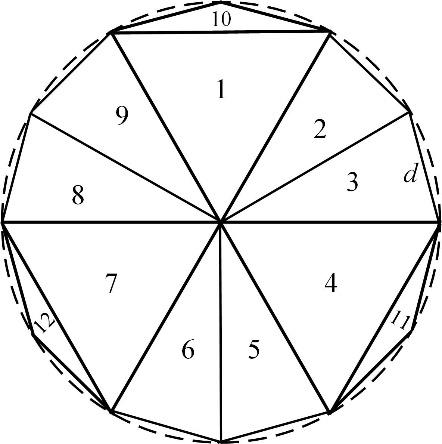
\includegraphics[width=0.2\linewidth]{fig2.jpg}
    \caption{}
    \label{fig:placeholder}
\end{figure}
\hfill(GATE EE 2025)

\begin{enumerate}
    \item
        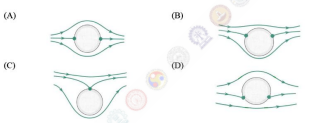
\includegraphics[width=0.2\linewidth]{fig3.jpg}
    \item 
        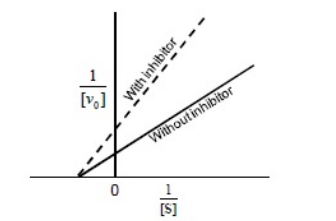
\includegraphics[width=0.2\linewidth]{fig 4.jpg}
    \item 
        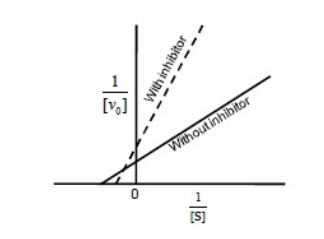
\includegraphics[width=0.2\linewidth]{fig 5.jpg}
    \item 
        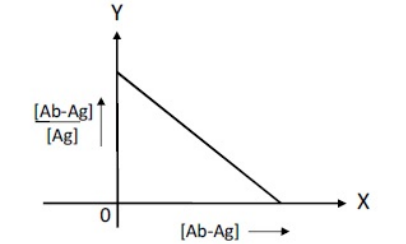
\includegraphics[width=0.2\linewidth]{fig 6.jpg}
        
\end{enumerate}

\item For a regular polygon having 10 sides, the interior angle between the sides of the polygon, in degrees, is  

\hfill(GATE EE 2025)

\begin{multicols}{4}
\begin{enumerate}
\item $396$
\item $324$
\item $216$
\item $144$
\end{enumerate}
\end{multicols}

\item Which one of the following numbers is exactly divisible by $(11^{13}+1)$?  

\hfill(GATE EE 2025)

\begin{multicols}{4}
\begin{enumerate}
\item $11^{26}+1$
\item $11^{33}+1$
\item $11^{39}-1$
\item $11^{52}-1$
\end{enumerate}
\end{multicols}

\item Oasis is to sand as island is to \underline{\hspace{2cm}}.  
Which one of the following options maintains a similar logical relation in the above sentence?  

\hfill(GATE EE 2025)

\begin{multicols}{4}
\begin{enumerate}
\item Stone
\item Land
\item Water
\item Mountain
\end{enumerate}
\end{multicols}

\item The importance of sleep is often overlooked by students when they are preparing for exams. Research has consistently shown that sleep deprivation greatly reduces the ability to recall the material learnt. Hence, cutting down on sleep to study longer hours can be counterproductive.  

Which one of the following statements is the CORRECT inference from the above passage?  

\begin{enumerate}
\item Sleeping well alone is enough to prepare for an exam. Studying has lesser benefit.
\item Students are efficient and are not wrong in thinking that sleep is a waste of time.
\item If a student is extremely well prepared for an exam, he needs little or no sleep.
\item To do well in an exam, adequate sleep must be part of the preparation.
\end{enumerate}

\item In the figure shown above, each inside square is formed by joining the midpoints of the sides of the next larger square. The area of the smallest square (shaded) as shown, in cm$^2$, is:  

    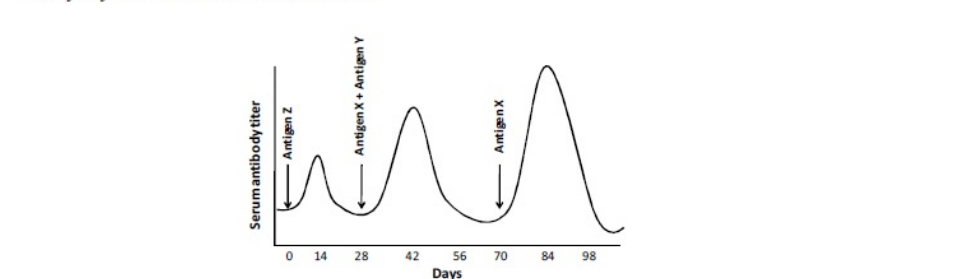
\includegraphics[width=0.2\linewidth]{fig 7.jpg}

\hfill(GATE EE 2025)

\begin{multicols}{4}
\begin{enumerate}
\item 12.50
\item 6.25
\item 3.125
\item 1.5625
\end{enumerate}
\end{multicols}

\item Let $X$ be a continuous random variable denoting the temperature measured. 
The range of temperature is $[0,100]$ degree Celsius and let the probability density function of $X$ be \begin{align*}
 f(x) = 0.01 \ \text{for } 0 \leq X \leq 100.     
\end{align*} 

The mean of $X$ is:

\hfill(GATE EE 2025)

\begin{multicols}{4}
\begin{enumerate}
\item 2.5
\item 5.0
\item 25.0
\item 50.0
\end{enumerate}
\end{multicols}

\item The number of students passing or failing in an exam for a particular subject are presented in the bar chart above. 
Students who pass the exam cannot appear for the exam again. Students who fail the exam in the first attempt must appear for the exam in the following year.Students always pass the exam in their second attempt. The number of students who took the exam for the first time in year 2 and in year 3 respectively, are \underline{\hspace{2cm}}\\
 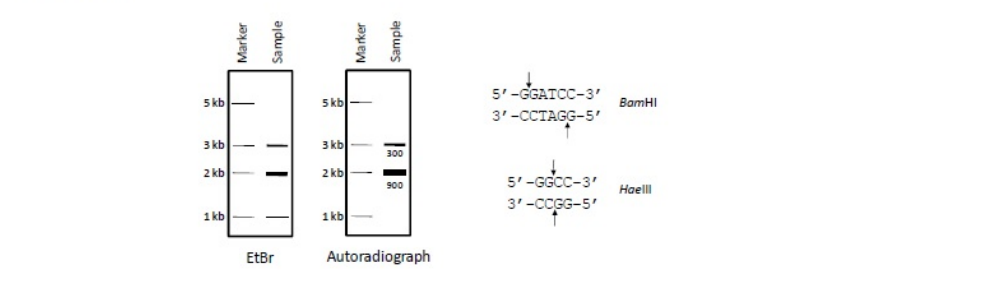
\includegraphics[width=0.4\linewidth]{figs/fig 8.jpg}
\hfill(GATE EE 2025)

\begin{multicols}{4}
\begin{enumerate}
\item 65 and 53
\item 60 and 50
\item 55 and 53
\item 55 and 48
\end{enumerate}
\end{multicols}

\item Seven cars P, Q, R, S, T, U and V are parked in a row not necessarily in that order.  
The cars T and U should be parked next to each other. The cars S and V also should be parked next to each other, whereas P and Q cannot be parked next to each other. Q and S must be parked next to each other.  
R is parked to the immediate right of V. T is parked to the left of U.  

Based on the above statements, the only INCORRECT option given below is:

\hfill(GATE EE 2025)

\begin{enumerate}
\item There are two cars parked in between Q and V.
\item Q and R are not parked together.
\item V is the only car parked in between S and R.
\item Car P is parked at the extreme end.
\end{enumerate}

\item Let the vector \begin{align*}
  \vec{v}=v_{1} \hat{i}+v_{2}\hat{j}+v_{3}\hat{k}   
\end{align*}be a differentiable
vector function of Cartesian coordinates $x, y, z$.  
The curl of the vector $\vec{v}$ is given by curl $\vec{v} =$ 

\hfill(GATE EE 2025)

\begin{multicols}{2}
\begin{enumerate}
\item $\left(\frac{\partial v_{3}}{\partial y} - \frac{\partial v_{2}}{\partial z}\right)\hat{i}
+ \left(\frac{\partial v_{1}}{\partial z} - \frac{\partial v_{3}}{\partial x}\right)\hat{j}
+ \left(\frac{\partial v_{2}}{\partial x} - \frac{\partial v_{1}}{\partial y}\right)\hat{k}$

\item $\left(\frac{\partial v_{2}}{\partial x} - \frac{\partial v_{1}}{\partial y}\right)\hat{i}
+ \left(\frac{\partial v_{3}}{\partial y} - \frac{\partial v_{2}}{\partial z}\right)\hat{j}
+ \left(\frac{\partial v_{1}}{\partial z} - \frac{\partial v_{3}}{\partial x}\right)\hat{k}$

\item $\left(\frac{\partial v_{3}}{\partial x} - \frac{\partial v_{2}}{\partial y}\right)\hat{i}
+ \left(\frac{\partial v_{1}}{\partial y} - \frac{\partial v_{3}}{\partial z}\right)\hat{j}
+ \left(\frac{\partial v_{2}}{\partial z} - \frac{\partial v_{1}}{\partial x}\right)\hat{k}$

\item $\left(\frac{\partial v_{2}}{\partial z} - \frac{\partial v_{3}}{\partial y}\right)\hat{i}
+ \left(\frac{\partial v_{3}}{\partial x} - \frac{\partial v_{1}}{\partial z}\right)\hat{j}
+ \left(\frac{\partial v_{1}}{\partial y} - \frac{\partial v_{2}}{\partial x}\right)\hat{k}$
\end{enumerate}
\end{multicols}

\item If $x$ is an integer with $x > 1$, the solution of  
\[
\lim_{x\to\infty}\left(\frac{1}{x}+\frac{2}{x^2}+\frac{3}{x^3}+\cdots+\frac{x+1}{x^{x}}\right)
\]
is

\hfill(GATE EE 2025)

\begin{multicols}{4}
\begin{enumerate}
\item Zero
\item 0.5
\item 1.0
\item $\infty$
\end{enumerate}
\end{multicols}

\item In a tyre axis system as defined by Society of Automotive Engineers, the
moment acting about z-axis is called

\hfill(GATE EE 2025)

\begin{multicols}{2}
\begin{enumerate}
\item aligning torque
\item over turning torque
\item rolling resistance moment
\item lateral moment
\end{enumerate}
\end{multicols}

\item Pitting is a process of

\hfill(GATE EE 2025)

\begin{enumerate}
\item mixing of pulses with red earth
\item mixing of pulses with edible oil
\item scratching of pulses by emery roller during its milling
\item beating of oil seeds for oil extraction
\end{enumerate}

\item During ploughing with a tractor mounted mould board plough, the mast of
three point hitch system would be

\hfill(GATE EE 2025)

\begin{enumerate}
\item inclined 5 to $20^\circ$ with horizontal
\item nearly vertical
\item parallel to the direction of travel of the tractor
\item parallel to the rear axle of the tractor
\end{enumerate}

\item The hydrologic reservoir routing methods use

\hfill(GATE EE 2025)

\begin{enumerate}
\item Bernoulli's equation only
\item hydrologic continuity equation only
\item Muskingum equation only
\item both the hydraulic momentum and hydrologic continuity equations
\end{enumerate}


\item While assessing the intensity of agricultural drought, a negative value ofaridity index indicates that the area is classified as

\hfill(GATE EE 2025)

\begin{multicols}{4}
\begin{enumerate}
\item severely arid
\item moderately arid
\item mildly arid
\item non-arid
\end{enumerate}
\end{multicols}

\item The approximate relationship between Sediment Delivery Ratio (SDR) and drainage area ($A$) shows that SDR varies

\hfill(GATE EE 2025)

\begin{multicols}{4}
\begin{enumerate}
\item directly with $A^{0.2}$
\item inversely with $A^{0.2}$
\item directly with $A$
\item inversely with $A$
\end{enumerate}
\end{multicols}

\item One-dimensional generalized heat conduction equation representing temperature distribution in a sphere, based on thermal conductivity $k$, specific heat capacity $C_p$, density $\rho$, and energy generation $E$, can be written as 

\begin{align*}
  \frac{1}{r^n}\frac{\partial}{\partial r}\left( r^k \frac{\partial T}{\partial r} \right) + E = \rho C_p \frac{\partial T}{\partial t},  
\end{align*}
where the value of $n$ is

\hfill(GATE EE 2025)

\begin{multicols}{4}
\begin{enumerate}
\item 1
\item 2
\item 3
\item 4
\end{enumerate}
\end{multicols}

\item In butter, the fishy flavor defect is due to the decomposition of

\hfill(GATE EE 2025)

\begin{multicols}{4}
\begin{enumerate}
\item $\alpha$-lactalbumin
\item $\beta$-lactoglobulin
\item casein
\item lecithin
\end{enumerate}
\end{multicols}

\item In a field test of drip irrigation system having an application efficiency of 90\%, the minimum, maximum and average flow rates are found to be 45 L h$^{-1}$, 65 L h$^{-1}$ and 50 L h$^{-1}$, respectively. The manufacturer's coefficient of variation of the emitter is 0.07. If there is one emitter per plant, the drip irrigation efficiency in percent is \underline{\hspace{2cm}}. [round off to 2 decimal places]

\item Trace of the matrix   \myvec
{3 & 2 & 1 & 4 \\
5 & 7 & 8 & 1 \\
2 & 4 & 6 & 7 \\
9 & 6 & 4 & 2} 
is \underline{\hspace{2cm}}.[in integer]

\hfill(GATE EE 2025)

\item The probabilities of A and B are given by P(A) = 0.35 and P(B) = 0.25, respectively. If A and B are mutually exclusive so that P(A $\cup$ B) = P(A) + P(B), then the value of P(A $\cup$ B) is \underline{\hspace{2cm}}.[round off to 3 decimal places]

\hfill(GATE EE 2025)

\item Stoichiometric air-fuel ratio of an SI engine is 14.7:1. If equivalence ratio ($\lambda$) is 0.92, the actual air-fuel ratio maintained during the engine operation is \underline{\hspace{2cm}}.[round off to 2 decimal places]

\hfill(GATE EE 2025)

\item While harvesting paddy with a self-propelled vertical conveyor reaper with a cutter bar of width 60 cm, the power required for cutting and propelling are measured to be 300 W and 350 W, respectively. If the power for conveying the cut crop is 50\% of the power required for cutting, the power required by the beater wheel unit of the vertical conveyor reaper in W will be \underline{\hspace{2cm}}.[answer in integer]

\hfill(GATE EE 2025)

\item A gear pump has a displacement of 120 cm$^3$ rev$^{-1}$ and it runs at 1500 rpm against a system pressure of 18 MPa. If the torque efficiency of the pump is 90\%, actual torque required to run the pump in N·m is \underline{\hspace{2cm}}.[round off to 2 decimal places]  
(Take $\pi = 3.14$)

\hfill(GATE EE 2025)

\item Useful soil reaction forces acting on a tractor drawn mould board plough during operation are 2.0 kN, 0.9 kN and 0.6 kN along longitudinal, transverse and vertical directions, respectively. The soil-metal friction angle is 25$^\circ$. Neglecting the effects of weight of the implement and the vertical soil reaction, the estimated draft in N is \underline{\hspace{2cm}}.{[round off to one decimal place]}

\hfill(GATE EE 2025)

\item Cohesionless soil is naturally deposited and makes a slope of infinite extent having slope angle of 25$^\circ$. If the effective angle of internal friction of this soil is 30$^\circ$, the factor of safety of slope is\underline{\hspace{2cm}}.{[round off to 2 decimal places]}

\hfill(GATE EE 2025)

\item A pump, discharging water at a rate of 80 L·s$^{-1}$, is used to irrigate 2 ha of land in 10 h. On irrigation, moisture content of the soil (on weight basis) in the root zone depth of 50 cm is increased from 18\% to 30\%. If bulk density of the soil is 1500 kg·m$^{-3}$, water application efficiency in per cent is \underline{\hspace{2cm}}. {[round off to 2 decimal places]}

\hfill(GATE EE 2025)

\item Pumping test is carried out at a constant discharge of 5400 L·min$^{-1}$ for 24 h in a main well of 30 cm diameter penetrated 25 m below the static water table. The water level in observation wells located at 30 m and 90 m away from the main well are lowered by 1.11 m and 0.53 m, respectively. Considering steady state flow condition, drawdown estimated in the main well in m is.\underline{\hspace{2cm}}.{[round off to 2 decimal places] (Take $\pi = 3.14$)}

\hfill(GATE EE 2025)

\item The observed concentrations of magnesium (Mg$^{2+}$), sodium (Na$^{+}$), and bicarbonate (HCO$3^-$) in saturated extract of a soil sample taken from the root zone are 5.68 meq·L$^{-1}$, 9.90 meq·L$^{-1}$, and 11.20 meq·L$^{-1}$, respectively. If the concentration ratio of HCO$_3^-$/Ca$^{2+}$ is 2.8, the sodium adsorption ratio is \underline{\hspace{2cm}} .  

\hfill(GATE EE 2025)

\item Fresh potatoes of mass 1000 kg are dried from 14\% to 93\% total solids. If 7\% of original potatoes is lost in peeling, the product yield from fresh potatoes in percent is \underline{\hspace{2cm}}. {[answer in integer]}

\hfill(GATE EE 2025)

\item In an ordinary chimney, the draught is 12 mm of water column. Assuming density of water to be 1000 kg·m$^{-3}$, the pressure difference between the outside air and gas at the base of the chimney in Pa is \underline{\hspace{2cm}}.{[round off to one decimal place]}

\hfill(GATE EE 2025)

\item A ball mill of 200 cm diameter grinds solid materials while operating with 10 cm size balls. If the same ball mill is used for wet grinding, charged with 20 cm diameter balls, the change in the operating speed in rpm is \underline{\hspace{2cm}}.{[round off to 2 decimal places] (Take $\pi = 3.14$ and $g = 9.81$ m·s$^{-2}$)}

\hfill(GATE EE 2025)

\item Rushton turbine having an impeller diameter of 20 cm and operating at a stirrer speed of 200 rpm is used in a mixing tank. If the tank receives air at a volumetric flow rate of 0.2 m$^{3}$·min$^{-1}$, the non-dimensional Froude Number, $Fr$ is \underline{\hspace{2cm}}.{[round off to 2 decimal places]}

\hfill(GATE EE 2025)

\item Solution of the differential equation $y'' + y' + 0.25y = 0$ with the initial values $y(0) = 3.0$ and $y'(0) = -3.5$ is.

\hfill(GATE EE 2025)

\begin{multicols}{4}
\begin{enumerate}[label=(\Alph*)]
\item $y = (3 - 2x)e^{0.5x}$
\item $y = (3 - 2x)e^{-0.25x}$
\item $y = (3 - 2x)e^{-0.5x}$
\item $y = (2 - 3x)e^{-0.5x}$
\end{enumerate}
\end{multicols}

\item A shear annulus with inner and outer diameters of 240 mm and 300 mm, respectively is used to measure shear strength of soil in the field. When it is inserted into the soil and rotated, the torque measured at the soil failure is 50 N·m. Shear strength of the soil in kPa is. (Take $\pi = 3.14$)

\hfill(GATE EE 2025)

\begin{multicols}{4}
\begin{enumerate}
\item 14.49
\item 18.94
\item 21.54
\item 28.98
\end{enumerate}
\end{multicols}

\item A bushy crop with stem cross-sectional diameter 6 mm is to be cut by impact force at a height of 50 mm above the soil surface. Based on the entire stem cross-section, the modulus of elasticity is 1500 N·mm$^{-2}$ and ultimate tensile strength is 35 N·mm$^{-2}$. The force in N that would cause failure of the stem due to bending is . (Take $\pi = 3.14$)

\hfill(GATE EE 2025)

\begin{multicols}{4}
\begin{enumerate}
\item 14.84
\item 23.52
\item 29.69
\item 44.53
\end{enumerate}
\end{multicols}

\item A solar panel has length of 1.3 m and width of 0.65 m. The solar cells cover 90\% of the panel area and its conversion efficiency is 13.7\%. For a total solar radiation of 750 W·m$^{-2}$, the panel output voltage is 18 V at its maximum power output. If two such panels are connected in series to supply power to run a thresher, the current in A that can be supplied by the two panels at the maximum power output is.

\hfill(GATE EE 2025)

\begin{multicols}{4}
\begin{enumerate}
\item 2.17
\item 3.01
\item 4.34
\item 6.08
\end{enumerate}
\end{multicols}

\item A fertilizer drill with a row to row spacing of 40 cm, discharges 38 g of fertilizer per row per revolution of the metering wheel. The metering wheel is driven through a chain transmission system by ground wheel having 60 cm diameter. Neglecting skid of the ground wheel, for an application rate of 200 kg·ha$^{-1}$, the speed ratio of ground wheel to metering wheel will be . (Take $\pi = 3.14$)

\hfill(GATE EE 2025)

\begin{multicols}{4}
\begin{enumerate}
\item 1.40 : 1
\item 2.52 : 1
\item 3.64 : 1
\item 4.76 : 1
\end{enumerate}
\end{multicols}

\item A sample of wet sandy-clay loam soil of mass 135 kg is collected for laboratory tests. The wet density, water content (weight basis) and specific gravity of solids of this soil sample are 1.8 g·cm$^{-3}$, 18\%, and 2.7, respectively. The dry density (in g·cm$^{-3}$) and porosity (in per cent) of the soil sample, respectively, are .

\hfill(GATE EE 2025)

\begin{multicols}{4}
\begin{enumerate}
\item 1.53 and 43.50
\item 1.53 and 77.00
\item 1.65 and 43.50
\item 1.65 and 77.00
\end{enumerate}
\end{multicols}

\item It is proposed to develop bench terraces in an area having land slope of 10\%. If the vertical interval between the bench terraces is 2.5 m and the batter slope is 100\%, working width (in m) and the area lost for cultivation (in per cent), respectively will be.

\hfill(GATE EE 2025)

\begin{multicols}{4}
\begin{enumerate}
\item 22.50 and 0.05
\item 25.00 and 0.50
\item 22.50 and 10.45
\item 25.00 and 10.45
\end{enumerate}
\end{multicols}

\item While carrying out a traverse survey $ABCDA'$ using a theodolite with the originating station A, the departures and latitudes of the lines, as obtained, are shown in the figure (not drawn to scale). It is seen that, due to the observational errors, the originating station A and its computed station A' are not the same. For this survey, the 'closing error' in m is .

 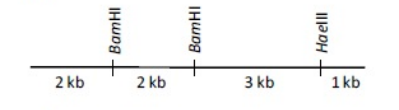
\includegraphics[width=0.3\linewidth]{fig 9.jpg}
\hfill(GATE EE 2025)

\begin{multicols}{4}
\begin{enumerate}
\item 6.33
\item 7.62
\item 33.73
\item 35.21
\end{enumerate}
\end{multicols}

\item The shape of the Instantaneous Unit Hydrograph (IUH) of a catchment is an isosceles triangle with a peak of 60 m$^{3}$·s$^{-1}$ and time to peak of 3 h. If the constant baseflow is 7.5 m$^{3}$·s$^{-1}$, the peak of the 3 h Unit Hydrograph (UH) in m$^{3}$·s$^{-1}$ is .

\hfill(GATE EE 2025)

\begin{multicols}{4}
\begin{enumerate}
\item 43.33
\item 50.83
\item 52.50
\item 60.00
\end{enumerate}
\end{multicols}

\item Match the following hulling mechanism in column 1 with the corresponding machine in column 2.  

\begin{center}
\begin{tabular}{|c|l|c|l|}
\hline
\textbf{Column 1} & & \textbf{Column 2} & \\ \hline
P & Shear and compression & 1 & Blade type emery scourer \\ \hline
Q & Friction and abrasion & 2 & Horizontal \textit{Gola} machine \\ \hline
R & Shear, compression and friction & 3 & Rubber roll dehusker \\ \hline
S & Impact, abrasion and friction & 4 & Under runner disc sheller \\ \hline
\end{tabular}
\end{center}

\hfill(GATE EE 2025)

\begin{multicols}{2}
\begin{enumerate}
\item P-3, Q-2, R-4, S-1
\item P-3, Q-1, R-2, S-4
\item P-3, Q-1, R-4, S-2
\item P-4, Q-3, R-1, S-2
\end{enumerate}
\end{multicols}

\item Match the correct items in column 1 with column 2

\begin{center}
\begin{tabular}{|c|l|c|l|}
\hline
\textbf{Column 1} & & \textbf{Column 2} & \\
\hline
P & Pipe-in-pipe heat exchanger & 1 & Cooling of air \\
Q & Shell and tube heat exchanger & 2 & Simultaneous co-current and counter current heat exchange \\
R & 1-2 shell and tube heat exchanger & 3 & Large flow rate \\
S & Cross flow heat exchanger & 4 & Small heat exchange area \\
\hline
\end{tabular}
\end{center}

\hfill(GATE EE 2025)

\begin{multicols}{2}
\begin{enumerate}
\item P-1, Q-2, R-4, S-3
\item P-2, Q-3, R-4, S-1
\item P-3, Q-4, R-2, S-1
\item P-4, Q-3, R-2, S-1
\end{enumerate}
\end{multicols}

\item A 30 $\mu$m thick membrane having 3 m$^2$ surface area is used to separate NaCl from a solution at steady state condition. The mass transfer coefficient of NaCl at the solution side is 1$\times$10$^{-6}$ ms$^{-1}$ and that at the other side of the membrane is 3$\times$10$^{-7}$ ms$^{-1}$. Concentration of NaCl in the solution is 0.03 g(100 mL)$^{-1}$ and that on the other side of the membrane is assumed to be zero. Permeability of the membrane is 0.9$\times$10$^{-6}$ ms$^{-1}$. The rate of removal of the NaCl by the membrane in gh$^{-1}$ is

\hfill(GATE EE 2025)

\begin{multicols}{4}
\begin{enumerate}
\item 0.73
\item 0.81
\item 0.86
\item 0.93
\end{enumerate}
\end{multicols}

\item In a size reduction operation, the power required to crush 2 ton of feed material per hour is 7.2 kW. Eighty per cent of the feed and product material pass through 4.75 mm and 0.5 mm sieve openings, respectively. The work index of the material is

\hfill(GATE EE 2025)

\begin{multicols}{4}
\begin{enumerate}
\item 6.5
\item 7.4
\item 11.9
\item 14.8
\end{enumerate}
\end{multicols}

\item A nine-member committee of an Agricultural University consists of 4 B. Tech., 3 M. Tech., and 2 Ph. D. students. It is decided to remove three students from the committee at random. The probability of removing 2 students from the same category and the third one from any other category is \underline{\hspace{2cm}}.{[round off to 3 decimal places]}


\item Summation of eigenvalues of a matrix 
\myvec{
4 & 1\\
3 & 6}

is \underline{\hspace{2cm}}.{[round off to the nearest integer]}

\hfill(GATE EE 2025)

\item During operation of a two-wheel drive tractor with a total weight of 20 kN in pure sandy soil (angle of internal friction is 26.5$^\circ$), the weight distribution at the front and rear axles are found to be 35\% and 65\%, respectively. If an extra weight of 2.5 kN is added to each of the rear wheels, the change in maximum thrust developed by the tractor in per cent will be \underline{\hspace{2cm}}.{[round off to 2 decimal places]}

\hfill(GATE EE 2025)

\item A tractor PTO driven rotavator with a rotor radius 30 cm has 20 L-shaped blades each of width 12 cm. These blades are fixed at a radial distance of 7 cm from the center of the rotor shaft to the brackets attached to the rotor shaft. When this rotavator is operated at a forward speed of 4.5 kmh$^{-1}$ and at a depth of 12 cm, the resultant soil force of 150 N tangential to the rotor circumference acts at the middle of the blade width. The torsional moment acting on the blade in Nm is \underline{\hspace{2cm}}.{[round off to one decimal place]}

\hfill(GATE EE 2025)

\item Fixed cost per year and variable cost per hour of a tractor were estimated based on its annual usage of 800 h. The total cost of operation was found to be Rs. 540 per hour. It was later re-estimated and found that total cost of operation would be Rs. 510 per hour, if the annual hours of use were increased to 1000 h. Considering all the components of annual usage cost to be the same, the variable cost in Rs. per hour would be \underline{\hspace{2cm}}.{[answer in integer]}

\hfill(GATE EE 2025)

\item Two meshed involute gears transmit 1.0 kW power. The pressure angle is 20$^\circ$ and the pitch circle diameter of the large gear rotating at a speed of 600 rpm is 20 cm. If only a pair of teeth are in contact at a time, the total force acting between the meshed teeth in N will be \underline{\hspace{2cm}} {[round off to one decimal place]}(Take $\pi = 3.14$)

\hfill(GATE EE 2025)

\item A horizontal axis lift type wind rotor of diameter 4 m is used to run a pump at a wind velocity of 15 kmh$^{-1}$ at standard atmospheric pressure and temperature (density of air is 1.23 kgm$^{-3}$). If velocity of wind leaving a rotor blade is reduced to one-third of the approaching wind velocity, the thrust acting on the blade of the wind rotor in N is\underline{\hspace{2cm}}.{[round off to 2 decimal places]}

\hfill(GATE EE 2025)

\item A small watershed receives rainfall of 90 mm in a day. For this watershed, irrespective of the land use, the amount of initial abstraction can be considered as 25\% of the potential maximum retention (S) of soil. Initially, the entire watershed was under forest with S = 136 mm, which was converted into cultivated land with S = 64 mm. The change in the daily runoff volume due to this land use alteration for this specific rainfall event in percent is \underline{\hspace{2cm}}.{[round off to one decimal place]}

\hfill(GATE EE 2025)

\item The most economical trapezoidal channel section with 1:1 (horizontal:vertical) side slope is designed to carry a maximum of 40 cm depth of water at its full capacity. If the bed slope of the channel is 1:2500 and the Manning's roughness coefficient of channel section is 0.01, the estimated discharge capacity of the channel in m$^3$s$^{-1}$ is \underline{\hspace{2cm}}.{[round off to 2 decimal places]}

\hfill(GATE EE 2025)

\item A windbreak, 15 m in height and 200 m in length, is established to protect the land from wind erosion in an arid area. The minimum wind velocity at the height of 15 m above the ground required to move the most erodible soil fraction is 9.6 ms$^{-1}$. If 5-year return period wind velocity at 15 m height is 16 ms$^{-1}$ and the wind direction deviates 20$^\circ$ from the line perpendicular to the windbreak, the area protected by the windbreak in ha is \underline{\hspace{2cm}}.{[round off to 2 decimal places]}

\hfill(GATE EE 2025)

\item Water is discharged from a tank through a rectangular orifice of width 1.5 m and height 1.2 m. The water level in the tank is 3.5 m above the top edge of the orifice. If the coefficient of discharge of this orifice is 0.62, the discharge through the orifice in m$^3$s$^{-1}$ is \underline{\hspace{2cm}}.{[round off to 2 decimal places]} 
(Take acceleration due to gravity, g = 9.81 ms$^{-2}$)

\hfill(GATE EE 2025)

\item Two fully penetrating wells are dug 1.4 km apart in a homogenous confined aquifer. The difference in their piezometric levels is 4.0 m. The groundwater flow is steady and unidirectional. If the aquifer has a hydraulic conductivity of 3.5 mday$^{-1}$ and effective porosity of 40\%, the time taken for water to move from one well to the other in days is \underline{\hspace{2cm}}.{[in integer]}

\hfill(GATE EE 2025)

\item Food cans are sterilized in a retort to inactivate \textit{Clostridium botulinum}. Lethal rate (F$0$) of this food material is 150 s at a reference temperature of 121.1 $^\circ$C. Temperatures at the slowest heating location inside the food can are measured as 71.1 $^\circ$C, 98.9 $^\circ$C and 110 $^\circ$C after 20, 40 and 70 min, respectively. The actual process time in minutes that is required for equivalent sterilization at 121.1 $^\circ$C is \underline{\hspace{2cm}}.{[round off to 2 decimal places]}

\hfill(GATE EE 2025)

\item Molecular masses of water and air are 18.02 and 28.97 kg(kg mol)$^{-1}$, respectively. Air in a room is at 40 $^\circ$C under a total pressure of 101.3 kPa absolute and contains water vapour at a partial pressure of 4.0 kPa. If saturated vapour pressure of water at 40 $^\circ$C is 7.37 kPa, the relative humidity of this air in per cent is \underline{\hspace{2cm}}.{[round off to 2 decimal places]}

\hfill(GATE EE 2025)

\item A cylindrical storage bin with an internal diameter of 4 m and a height of 16 m is completely filled with paddy having bulk density of 640 kgm$^{-3}$. The angle of internal friction between grain and bin wall is 30$^\circ$ and the ratio of horizontal to vertical pressure is 0.4. When the grain fills from 8 m in height to 16 m in height, the lateral pressure increases by a multiple of \underline{\hspace{2cm}}.{[round off to 2 decimal places]}

\hfill(GATE EE 2025)

\item An air screen grain cleaner unit of capacity one tonh$^{-1}$ with two screens was evaluated with a feed containing 8.5\% impurities. During the operation, the clean grain at blower outlet, overflow of 1$^{st}$ screen and underflow of 2$^{nd}$ screen were found to be 0.3\%, 1.2\% and 0.8\%, respectively. If the clean grain contains 0.6\% of impurities, the cleaning efficiency of the cleaner unit in per cent would be \underline{\hspace{2cm}}.{[round off to one decimal place]}

\hfill(GATE EE 2025)

\item One side of a solid food block of 10 cm thickness is subjected to a heating medium having a film heat transfer coefficient of 70 W(m$^2$$^\circ$C)$^{-1}$. The other side of the food block is being cooled by a medium having a film heat transfer coefficient of 100 W(m$^2$$^\circ$C)$^{-1}$. The food block is having a thermal conductivity of 0.2 W(m$^\circ$C)$^{-1}$ and the contact area of the block available for heat transfer is 1 m$^2$. Heat transfer rate in the block at steady state is 100 Js$^{-1}$. The temperature difference between the two sides of the block in $^\circ$C is \underline{\hspace{2cm}}.{[round off to 2 decimal places]}

\hfill(GATE EE 2025)

\end{enumerate}

\end{document}

